\chapter{Zyxel GS1920-8HP} \label{zyxel}

The Zyxel GS1920-8HP model is a managed switch with 10 available ports for interconnectivity. The Zyxel switch is what powers every Raspberry Pi 3B+ machine using \gls{poe}, with port 9 providing Internet access.

\begin{figure}[H]
    \centering
    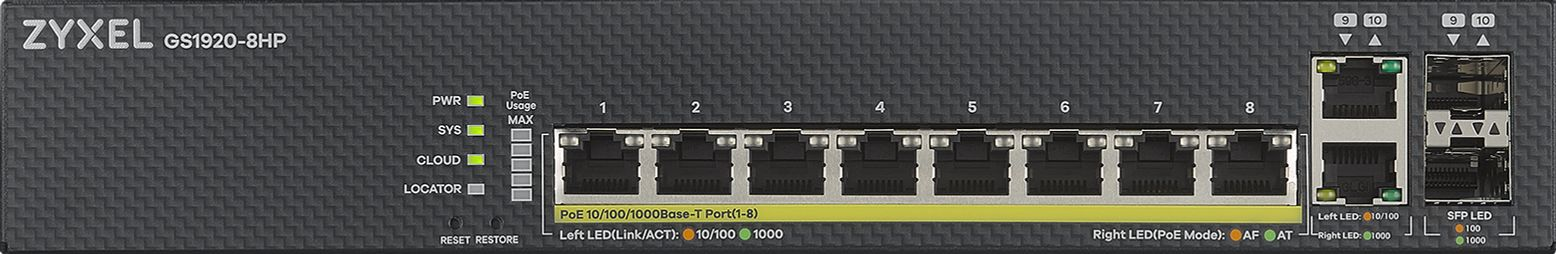
\includegraphics[width=1.0\linewidth]{zyxel}
    \captionsetup{width=1.0\linewidth}
    \caption{The front of the Zyxel GS1920-8HP managed switch.}
    \label{fig:zyxel}
\end{figure}


\section{VLAN Setup}

In order to logically separate two subnets on a single switch, as illustrated in \ref{fig:network_topology}, two \gls{vlan}s must be set up. This can easily be done through the switch's graphical user interface that can be accessed in several ways as shown in the official \href{https://www.zyxel.com/support/download_landing/product/gs1920_series_18.shtml?c=gb&l=en&pid=20130521174252&tab=Quick_Start_Guide&pname=GS1920%20Series}{quick start guide.}. In short, connect a computer to the Zyxel switch with an Ethernet cable, set a static IP of 192.168.1.10, and access the graphical user interface in a web browser by visiting the address 192.168.1.1.

The default username and password for Zyxel GS1920-8HP is \lstinline{admin} and \lstinline{1234}, respectively. Once logged in, go to \lstinline{Advanced Application -> VLAN -> VLAN Configuration -> Static VLAN Setup}.

\begin{figure}[H]
    \centering
    \begin{subfigure}{0.5\linewidth}
        \centering
        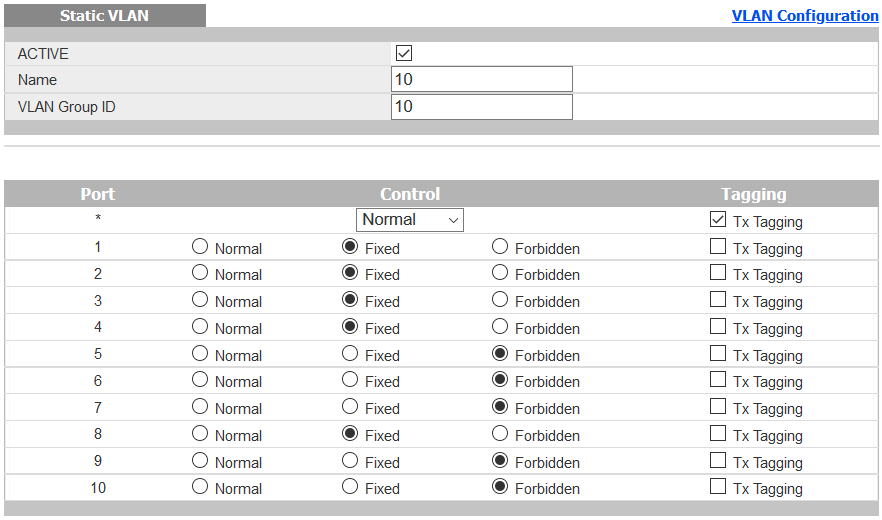
\includegraphics[width=1.0\linewidth]{vlan10}
        \caption{VLAN 10}
        \label{fig:vlan10}
    \end{subfigure}%
    \begin{subfigure}{0.5\linewidth}
        \centering
        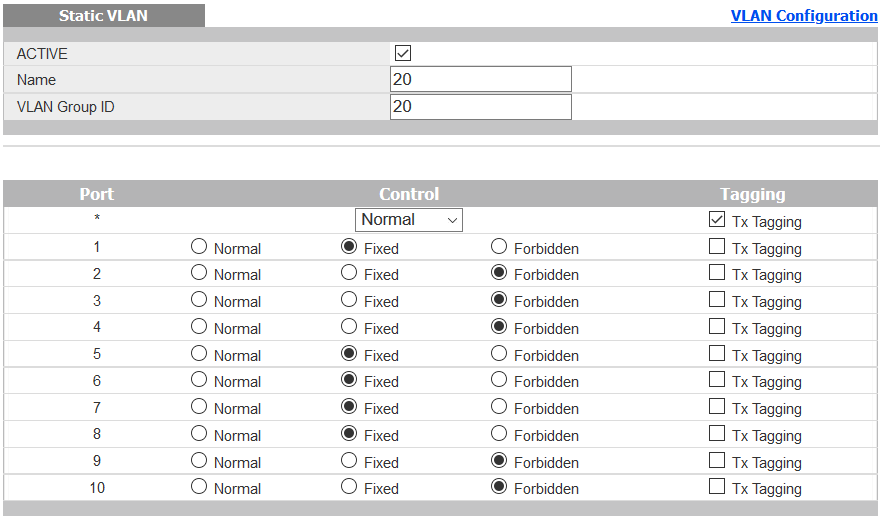
\includegraphics[width=1.0\linewidth]{vlan20}
        \caption{VLAN 20}
        \label{fig:vlan20}
    \end{subfigure}
    \caption{The configuration for the two \gls{vlan}s on Zyxel GS1920-8HP.}
    \label{fig:vlans}
\end{figure}

Create two \gls{vlan}s as shown above, confirming each creation with the \lstinline{Add} button. When done, persist the changes with the \lstinline{Save} button in the top right corner.